\documentclass[12pt,twoside,a4paper]{article}
\usepackage{hyperref}
\usepackage{graphicx}
\graphicspath{ {../img/} }
\usepackage[left=2cm, right=2cm, top=2.5cm, bottom=3cm]{geometry}
\title{Operativni sistem Linux}
\author{Vojislav Lazić}
\date{February 2019}
\tolerance=1
\emergencystretch=\maxdimen
\hyphenpenalty=10000
\hbadness=10000
	\begin{document}
    \thispagestyle{empty}
    \noindent
    Šesta beogradska gimnazija\\
    Milana Rakića 33\\
    Beograd
    \vfill
    \begin{center}
        \begin{Large}
        Maturski rad iz informatike\\
        \bigskip 
        \end{Large}
        {\Huge
        Operativni sistem Linux}
    \end{center}
    \vfill
    \noindent Mentor: \hfill Učenik:\\
    Olivera Mihailović \hfill Vojislav Lazić IV$_{9}$\\
    Profesor informatike
    \vfill
    \begin{center}
        Beograd, jun 2019.
    \end{center}
\thispagestyle{empty}
\newpage
\renewcommand{\contentsname}{Sadržaj}
\tableofcontents
\newpage
\section{Istorija Linuxa}
\indent Za stvaranje Linux-a bilo je potrebno nekoliko komponenti, najvažnija od kojih je Unix. Unix su stvorili Ken Tompson i Denis Riči. Njih dvojica, zajedno sa timom inženjera u Belovim laboratorijama, su radili na Multics sistemu (\textbf{M}ultiplexed \textbf{I}nformation and \textbf{C}omputing \textbf{S}ervice), pravljen sa idejom da bude sistem koji može da radi više poslova u isto vreme. Tompson i Riči su u  tom periodu počeli da rade na svom sopstvenom sistemu, zasnovan na Multics-u, po imenu Unix, prvi put objavljen 1970. godine. Kasnije, kad je C programski jezik, koji je Riči napisao zajedno sa Brajanom Kernigenom, postao dovoljno razvijen, Unix je potpuno prepisan u C-u, što je pomoglo njegovom rasprostranjenju u razne akademske institucije i poslove. Zbog promenljive i prilagodljive prirode Unix-a, razni univerziteti su počeli da prave svoje verzije Unix-a, jedan od najpopularnijih je bio BSD (\textbf{B}erkeley \textbf{S}oftware \textbf{D}istribution), koji je još u upotrebi danas.\\

1983. godine, Ričard Metju Stalman je započeo GNU projekat, namenjen da bude slobodna alternativa za Unix. Do ranih 90-ih, napisano je dovoljno softvera da se napravi citav operativni sistem. Jedino što je nedostajalo je ``kernel'' ili ``jezgro'' operativnog sistema, deo koji bi trebao sve ostale komponente da spoji. GNU je imao, i još ima, u pravljenju svoji kernel, GNU Hurd, ali nikad nije završen. Postojao je i kernel zasnovan na BSD-u, ali bez dovoljno funkcionalnosti.\\

Nedostatak besplatnog i korisnog kernel-a, je nerviralo Linusa Torvaldsa, pa je stoga odlučio da napiše svoji sopstveni. Torvalds je bio upoznat već sa Minix-om i sa GNU softverom i dok je bio student informatike na Univerzitetu u Finskoj je počeo da radi na projektu koji bi kasnije postao Linux kernel. 25.-og avgusta 1991. godine, Torvalds je postavio na Usenet newsgroup-i o svom projektu. Nastavio je da bude projekat na kome je samo on radio, ali s vremenom je steklo sve više pažnje od drugih programera. Danas je preko 15000 programera  doprinelo preko 17 miliona linija koda.
\newpage
\begin{figure}[h]
	\centering
    \subfloat[Ken Tompson i Denis Riči, tvorci UNIX-a]{{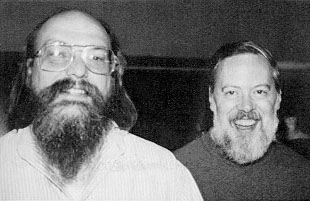
\includegraphics[height=3cm,width=4cm]{d_r} }}
    \hspace{1cm}
    \subfloat[Linus Torvalds, tvorac Linux-a]{{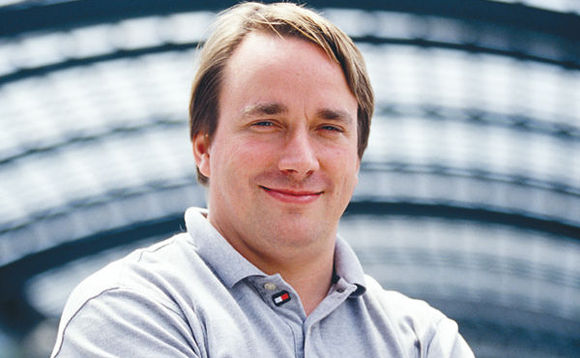
\includegraphics[height=3cm,width=4cm]{linus} }}
\end{figure}
\begin{figure}[h]
	\centering
    \subfloat[Flopi diskovi sa verzijom 0.12 Linux-a]{{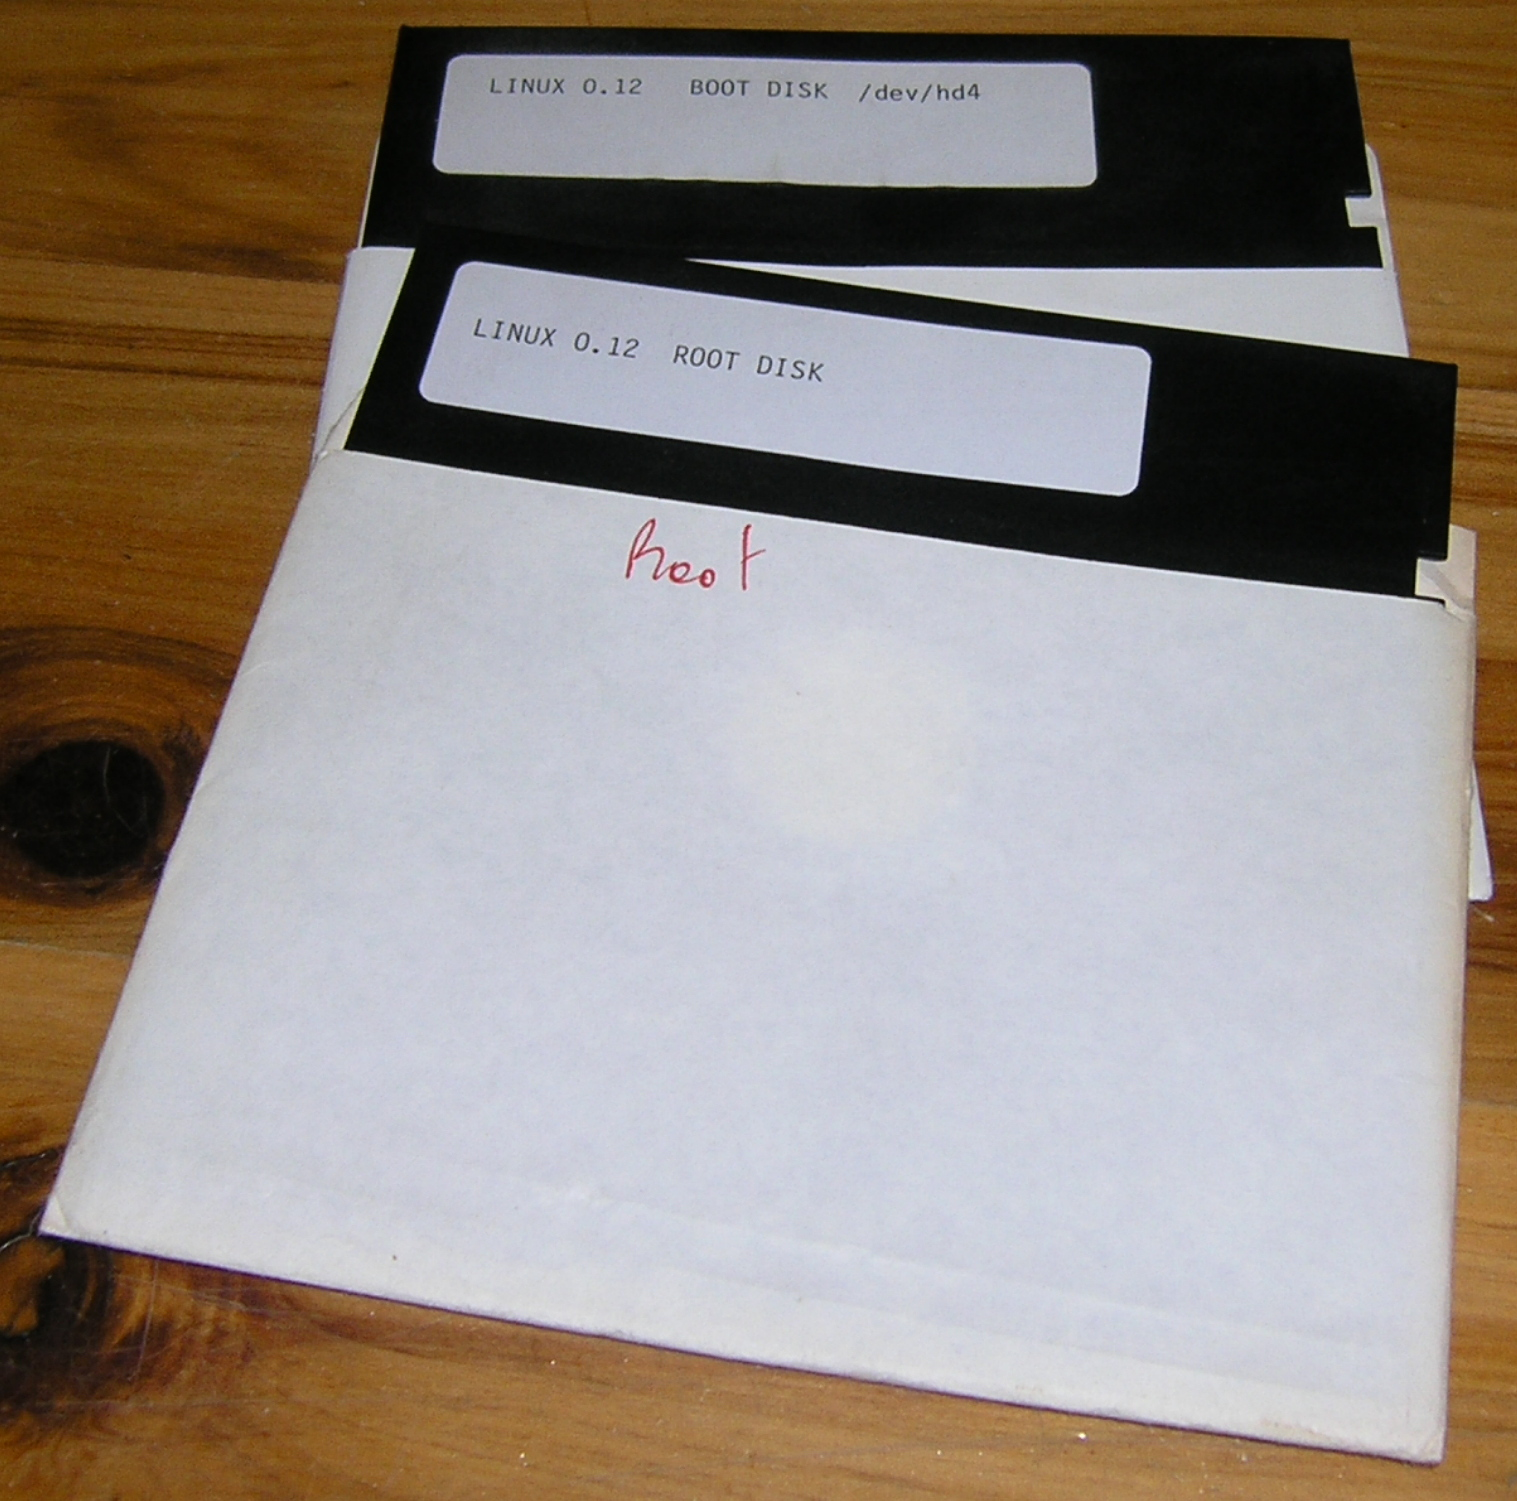
\includegraphics[height=3cm,width=4cm]{old_linux} }}
    \hspace{1cm}
    \subfloat[Ričard Metju Stalman, tvorac GNU-a]{{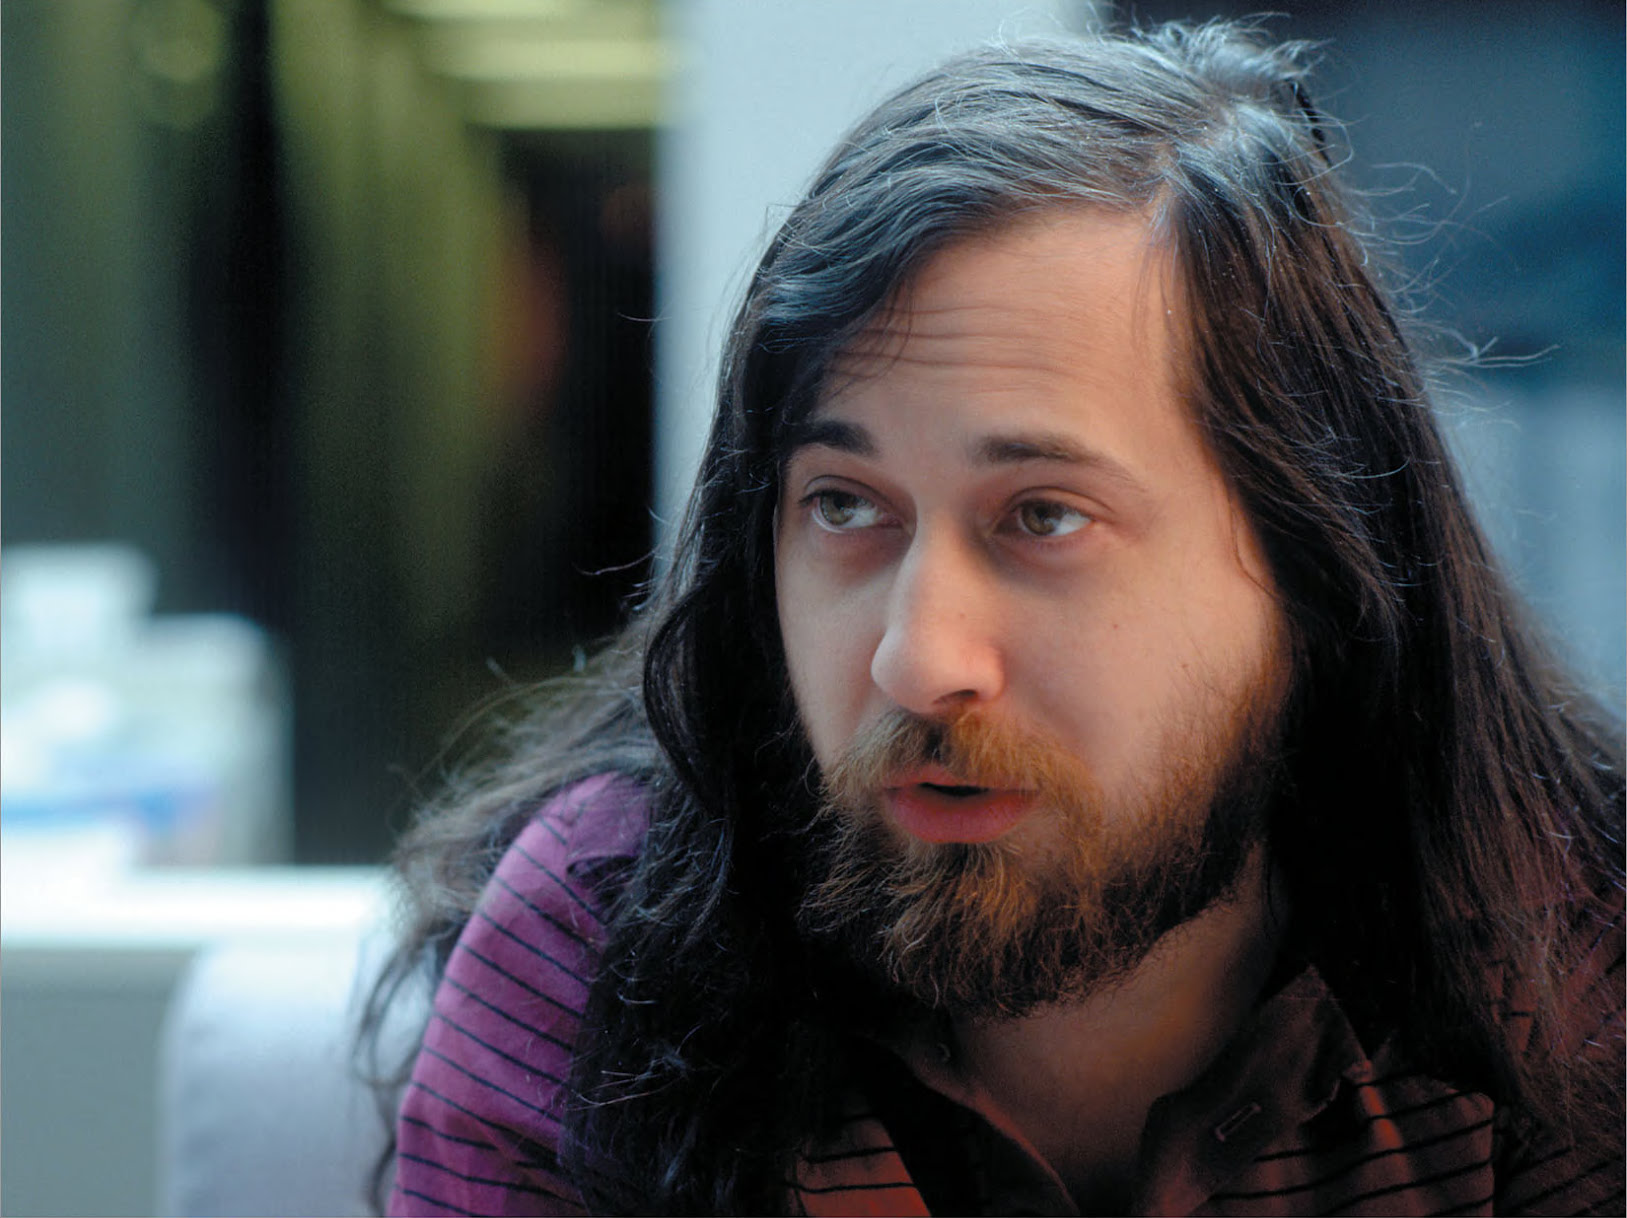
\includegraphics[height=3cm,width=4cm]{stallman} }}
\end{figure}
\begin{figure}[H]
	\centering
	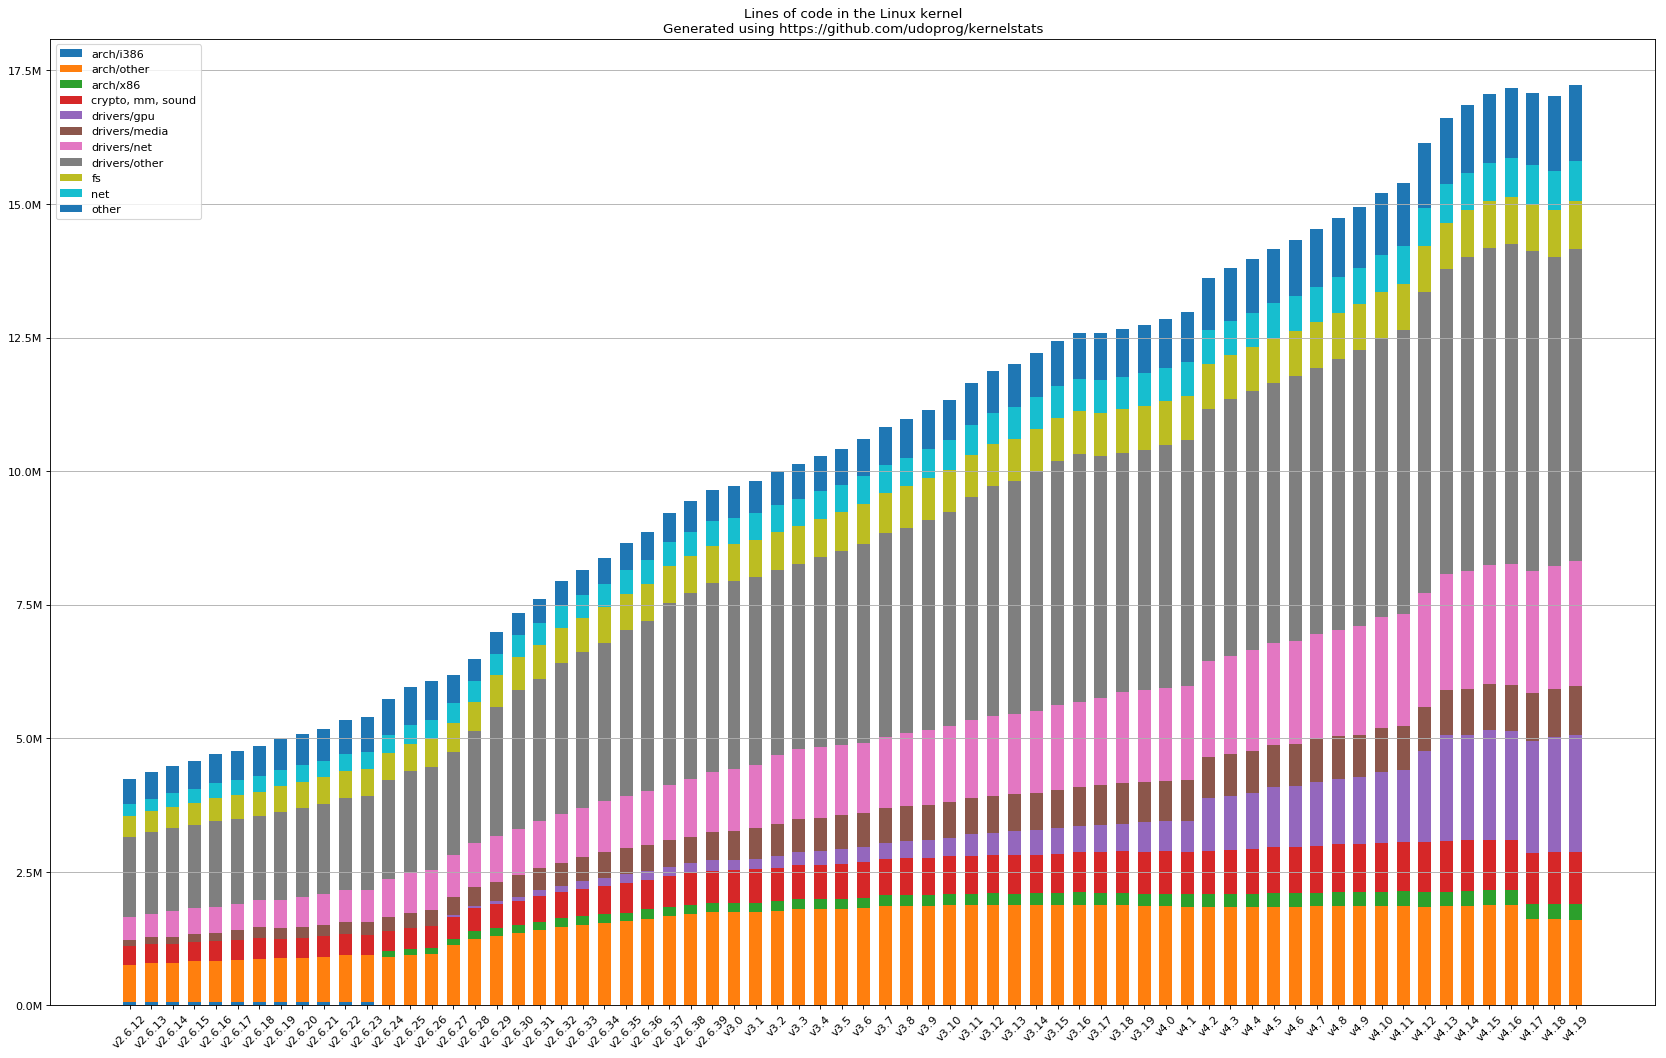
\includegraphics[width=\textwidth]{loc}
	\caption{Broj linija koda u Linux kernel-u od verzije 2.6.12 do danas}
\end{figure}
\newpage
\section{Komponente Linux sistema}
\subsection{Bootloader}
Boot loader je program koji se pokreće pre bilo kog operativnog sistema. Njegov posao je da nadje operativni sistem (ili više njih) i da ga pokrene. Na Linuxu postoji nekoliko bootloader-a:\begin{itemize}
\item GRUB (\textbf{GR}and \textbf{U}nified \textbf{B}ootloader) - najpopularniji, deo GNU programa napravljenih za GNU Hurd kernel.
\item LILO (\textbf{Li}nux \textbf{Lo}ader) - razvoj je prekinut jer nije podržavao sisteme sa više od jednog operativnog sistema.
\item SYSLINUX - skup neintenzivnih bootloader-a, najčešće se koriste za podizanje sistema sa drajvova malih kapaciteta, kao fleš drajv, DVD...
\end{itemize}


\subsection{Kernel}
Kernel je najvažniji i najosnovniji deo svakog operativnog sistema. Kernel je zadužen da pokrene svaku komponentu potrebu za korišćenje sistema, da služi kao posrednik u komunikaciji izmedju softvera i hardvera, i delova softvera medjusobno. Kernel je potreban tokom celog korišćenja računara, pa je stoga neophodno da on bude što manji i što efikasniji.\\
Osnovi delove kernela su obično:
\begin{itemize}
\item rasporednik - odredjuje kako će razni procesi koristiti snagu procesora
\item supervizor - odobrava kontrolu kompjutera procesu koji je na redu
\item rukovodilac zahteva - rukuje svim zahtevima upućenim kernelu
\item menadžer memorije - dodeljuje lokacije na memoriji procesima kernela
\end{itemize}
Postji 4 glavne kategorije kernel-a:
\begin{itemize}
\item monolitski - obično se nadju kod Unix-sličnih operativnih sistema, kao kod Linux-a i FreeBSD-a. Oni sadrže sve osnove funkcije OS-a i drajvere potrebne za korišćenje hardvera kao hard diskova, grafičkih kartica, printera. Moderni monolitski kernel-i imaju opciju da odrede koji moduli kernel-a će se koristiti, time smanjujući količinu koda kernel-a.
\item microkernel-i - imaju samo minimalan broj usluga kao menadžer memorije, sistem za komunikaciju izmedju procesa i menadžer procesa. Sve ostale funkcije su implementirane nezavisno od kernel-a. Primeri mikrokernel-a su GNU Herd, MINIX i Mac OS X.
\item hibridni - kompromis izmedju monolitskih i mikrokernel-a. Osimišljeni se pre nego što je otkriveno da su mikrokernel-i daleko efikasniji od hibridnih.
Eksperimentiše se sa exokernel-ima. Glavna razlika izmedju njih i ostalih vrsta kernel-a je što se jedino bave zaštitom harvera umesto menadžmentom hardvera. Ovim pristupom exokernel-i omogućuje programerima da bolje odrede kako najefikasnije da koriste raspoloživ hardver.
\end{itemize}
\cite{kernel}

\subsection{Daemoni}
Daemon je program na Linux sistemima koji radi u pozadini, bez direktne kontrole korisnika. Oni obično služe da odgovaraju na zahteve drugih kompjutera na mreži, ali takodje, da reaguju na softverske i hardverske promene na samom kompjuteru. Na primer, na daemon-e mogu da utiču odredjeno vreme ili datum, stvaranje fajla u specifičnom folderu, zahtev napravljen preko interneta, itd.
Daemon-i se vode u sistemu kao potprocesi "init" procesa, što je prvi proces koji se pokreče sa kompjuterom. Na većini novih Linux sistema, daemon-i se pale samo po potrebi i na zahtev jednog glavnog daemon-a - "xinetd". \cite{daemon}

\subsection{Shell}
Shell služi da obezbedi isključivo tekstualni "interfejs" za korisnika. Njegova primarna svrha je čita komande iz konzole i da ih pokrene. "Shell" ili "ljuska" se odnosi na to da je to spoljašnji sloj opertivnog sistema tj. shell je posrednik izmedju korisnika i unutrašnjih delova sistema. Osim za sa samo pokretanje programa, shell-ovi imaju sposobnost da usmeravaju output? jedne komande da bude korišćen kao input? druge komande - "piping" (prvo uvedeno još u UNIX-u) i takodje da služe kao programski jezik - sintaksa komandi može da se koristi za pisanje "shell skripti". Postoje razni shell-ovi, od kojih je najpopularniji "bash"(Bourne-again shell),  koji je nadogradnja na "sh"(Bourne shell) - originalni UNIX shell.
\subsection{X window sistem}
\subsection{Window menadzer}
\subsection{Desktop okruzenje}
\section{Osnovne komande u Linux-u}
Prednost GNU/Linux operativnih sistema nad drugim je ekstensivnost Linux-ovog \textit{terminal-a}. Terminal može da se koristi za svaku radnju na sistemu, kao manevrisanje kroz sistem, manipulacija fajlovima i folderima,  pokretanje i gašenje programa, kontrola trenutnih procesa, itd.\\
Dalje su objašnjene neke od osnovih Linux komandi.
\begin{itemize}
\item \texttt{pwd} - Svaki put kad se otvori shell, njegov rad je koncentrisan u jedan folder (ovaj folder je pri otvaranju terminal-a uvek ``home'' folder). \texttt{pwd} ispisuje folder u kome se trenutno radi. Skraćeno od ``print working directory''. 

\item \texttt{ls} - Ispisuje sve fajlove i podfoldere u zadatom folderu ili u trenutnom folderu ako ništa nije zadato. Na komande u Linux-u mogu da se dodaju opcije koje mogu dodatno da definišu kakav će tačno rezultat komande biti. Na primer, na \texttt{ls} komandu može da se doda \texttt{-a} opcija da bi se prikazali i skriveni fajlovi i folderi čija imena počinju sa tačkom. Skraćeno od ``list''.

\item \texttt{cd} - Menja folder u kome se trenutno radi na zadati folder, npr. \texttt{cd Documents}, ili vraća na \texttt{home} folder ako ništa nije zadato. Za vraćanje u prethodni folder koristi se \texttt{cd ..} (`` .. '' uvek označava folder relativno iznad trenutnog, dok `` . '' označava trenutni folder). Skraćeno od ``change directory''.

\item \texttt{mkdir} i \texttt{rmdir} - Pravi novi folder odnosno briše (pod uslovom da je prazan) zadati folder. Skraćeno od ``make directory'' i ``remove directory''.

\item \texttt{rm} - Briše zadati fajl. Može da se koristi sa opcijom \texttt{-r} (rekurzivno) da bi izbrisalo sadržaj zadatog foldera. Skraćeno od ``remove''.

\item \texttt{cp} - Kopira zadati fajl ili folder na datu lokaciju. Ova komanda uzima dva argumenta, lokacija fajla ili foldera koji želimo da kopiramo i lokacija gde želimo da ga kopiramo, odvojena razmakom. Na primer, \texttt{cp subfolder folder} (``subfolder'' će se kopirati na lokaciju /folder/subfolder). Skraćeno od ``copy''.

\item \texttt{mv} - Premešta fajl ili folder na datu lokaciju. Takodje uzima dva argumenta. Skrećeno od ``move''.

\item \texttt{cat} 	- Spaja i ispisuje sadržaj fajlova (ako je dat samo jedan fajl, ispisuje njegov sadržaj). Skraćeno od ``concatenate''.

\item \texttt{sudo} - Stavlja se kao prefiks bilo kojoj komandi da bi se pokrenula sa administratorskim ovalašćenjima. Za pokretanje je potrebna lozinka \textit{root} korisnika (administratora). Skraćeno od ``SuperUser do''.

\item \texttt{man} - Ispisuje upustva za korišćenje i sve opcije za bilo koju komandu. Skraćeno od ``manual''.
\end{itemize}
\begin{figure}[H]
	\centering
	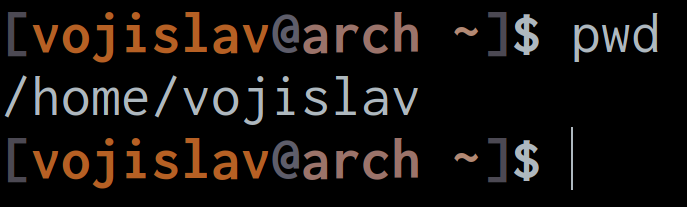
\includegraphics[scale=0.35]{pwd}
	\caption{Primer \texttt{pwd} komande}
\end{figure}
\begin{figure}[H]
	\centering
	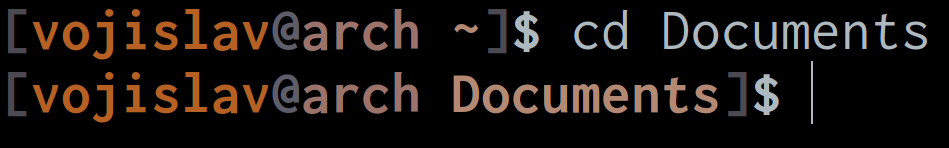
\includegraphics[scale=0.35]{cd}
	\caption{Primer \texttt{cd} komande}
\end{figure}
\begin{figure}[H]
	\centering
	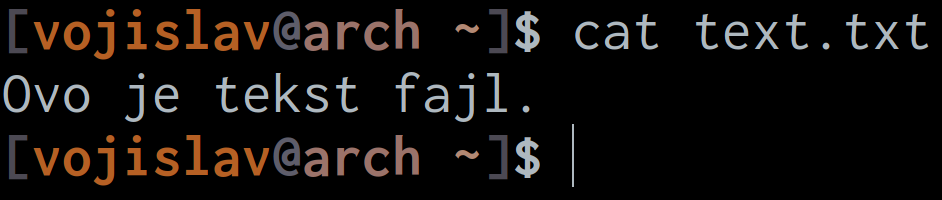
\includegraphics[scale=0.35]{cat}
	\caption{Primer \texttt{cat} komande}
\end{figure}
\nocite{linfo}
\renewcommand\refname{Literatura}
\bibliographystyle{unsrt}
\addcontentsline{toc}{section}{Literatura}

\bibliography{bib}
\end{document}